%!TEX program = lualatex
%!TEX encoding = UTF-8 Unicode  
%!TEX root = chapter03.tex  
\documentclass[main.tex]{subfiles} 
\begin{document} 
%----------------------------------------------------------------------------------------
%	CHAPTER 3
%----------------------------------------------------------------------------------------
\cleardoublepage 
\loadgeometry{marginlayout}  
\pagestyle{scrheadings} % Print headers again  
\KOMAoptions{
	headwidth=textwithmarginpar,
	headsepline=true,
	headsepline= 0.5pt,
	footwidth=textwithmarginpar,
}   
\onehalfspacing 
\setcounter{chapter}{2}
\chapter{Produit d'expression et identités}

%----------------------------------------------------------------------------------------
%	 
%----------------------------------------------------------------------------------------
% developpement simple, simplifcation, reduction
% former des expressions
% distributivité double
% identité remarquable
% factorisations simples
% démontrer avec les nombres entiers
% factorisations doubles pour problèmes du style : n^2-1 est il premier


%----------------------------------------------------------------------------------------
%	 
%----------------------------------------------------------------------------------------
%\newpage 
\section{Identités  et programmes de calcul}

Une \textbf{indentité} est une égalité dans laquelle apparaît une ou plusieurs lettres (dites variables) et qui reste vraie quelles que soient les valeurs prises par les variables. 

\marginnote{
	\begin{tBox}[leftline=false]
		interprétation simple : 
		$a$ paquets de $x$  + $b$ paquets de $x$   = $(a + b)$ paquets de $x$ !
	\end{tBox}
} 
\begin{tBox}[frametitle={Règle 1 : Axiome de distributivité}]
	Pour tout nombres relatifs $a$,$b$ et $x$ :  
	$ 	(a+b)\times x = (a\times x)+(b\times x)  	$ 
\end{tBox}
\begin{tBox}[frametitle={Règle 2}] Pour tout réel $a$ :  
	$a \times (-1) = (-a)$
\end{tBox}
\textbf{Développer} est une activité qui consiste à exploiter les 2 règles précédentes jusqu'à plus possible pour écrire une expression égale sous forme d'une \textbf{somme de termes}.
\begin{example}\hfill  
	\begin{enumerate}[label={$\Alph*=$}, leftmargin=*]  
		\item $- (2x-5) = -2x+5   $ 
	\end{enumerate} 
\end{example}  
\begin{tBox}[frametitle={La double distributivité}]
	Pour tout réels $a$,$b$,$x, y\in\mathbb{R}$ : 
	\begin{align*}
		(x + y)(a + b) &= x(a + b) + y(a + b)\\
		& = xa + xb + ya + yb
	\end{align*} 
\end{tBox} 
\begin{example} Pour $x\in \mathbb{R}$, développer :
	\begin{multicols}{2}
		\begin{enumerate}[label={$\Alph*(x)=$},leftmargin=*]
			\item   $(2x-2)\times  (3x-1)$
			\item   $(2x+5)+ (3x-1)$
			\item   $(2x+5)- (3x-1)$
			\item   $(-5x+1)   (3x-1)$
		\end{enumerate}
	\end{multicols}
\end{example}
%----------------------------------------------------------------------------------------
%	EXERCICES
%----------------------------------------------------------------------------------------

\newpage 
\loadgeometry{widelayout}  
\pagestyle{scrheadings} % Print headers again  
\KOMAoptions{
	headwidth=textwithmarginpar,
	headsepline=true,
	headsepline= 0.5pt,
	footwidth=textwithmarginpar,
} 
\onehalfspacing

\subsection{Exercices}


\begin{exercise}[\cancel{\faCalculator}] Calculer les expressions suivantes :\hfill 
	\begin{multicols}{3}
		\begin{enumerate}[label={$\alph*=$}, leftmargin=*] 
			\item $5+5\times 9$
			\item $(5+5)\times 9$
			\item $\tfrac{4}{4}+3$
			\item $\tfrac{4}{4+3}$
			\item $\tfrac{5}{7+4}$
			\item $4-\tfrac{5}{7}$   
			\item $6\times 3+7$ 
			\item $-6\times 3+7$
			\item $-6\times (3+7)$
			\item $-11\times 12-3$
			\item $2-8\times(-15)$
			\item $-6\times 11 +3$
		\end{enumerate}
	\end{multicols}
\end{exercise}
\begin{exercise}[\cancel{\faCalculator}, substitution] Calculer les expressions suivantes  :\hfill 
	\begin{multicols}{2}
		\begin{enumerate}[label={\alph*)}, leftmargin=*] 
			\item $-3+5x$ lorsque $x=-6$ 		
			\item $-3x-5$ lorsque $x=-2$ 		%   1
			\item $-9+7x$ lorsque $x=-7$ 		% -58
			\item $-8+9x$ lorsque $x=-8$ 		%  80
			\item $10+9x$ lorsque $x=-6$ 		% -44
			\item $(x+y)z$ lorsque $x=4$, $y=6$ et $z=-5$. 	%4
			\item $x^2-yz$ lorsque $x=-1$, $y=-2$ et $z=9$. 	% 
			\item $xy+z^2$ lorsque $x=10$, $y=-7$ et $z=-5$. 	% 
		\end{enumerate}
	\end{multicols}
\end{exercise}
\begin{example}\hfill 
	\begin{enumerate}[label=\alph*),leftmargin=*]
		\item $(2+4)\times (x+2)$ est une \BoiteFlash{} 
		\item $7+2\times x+3$  est une \BoiteFlash{} 
		\item Quand on multiplie deux nombres, chaque nombre est un \BoiteFlash{}  du produit.
		\item Quand on ajoute deux nombres, chaque nombre est un \BoiteFlash{}  de la somme.
	\end{enumerate}
\end{example} 
\begin{exercise}[Somme ou produit ?] Cocher la bonne réponse. 
	
	\noindent\parbox{0.48\linewidth}{
		\QCM[VF,Alterne,Stretch=1.1, Largeur=1.5cm, NomV=Produit,NomF=Somme]{%
			$2-5x$&2,%
			$2+x\times 3 +5$&2,%
			$(5+1)^2$&1,%
			$(3x-2)+(5x-4)$&2,%
		} 
	}\hfill
	\parbox{0.50\linewidth}{
		\QCM[VF,Alterne,Stretch=1.1, Largeur=1.5cm, NomV=Produit,NomF=Somme]{%
			$(2x-1)(8x+2)$&1,%
			$5x+1$&2,%
			$x^2-25$&2,%
			$(x-1)(x+1)$&1,% 
		}
	} 
\end{exercise}  
\begin{exercise}[Identités A] \hfill 
	\begin{enumerate}[label=\alph*),leftmargin=*]
		\item Montrer que les valeurs $x=1$, $x=3$ et $x=5$  rendent l'égalité suivante vraie :
		\setlength{\abovedisplayskip}{5pt}
		\setlength{\belowdisplayskip}{5pt}
		\[ 7(x-8)-3(x-20)=4(x+1)\]
		\item Montrer que pour tout $x$   on a	$ 7(x-8)-3(x-20)=4(x+1) $
	\end{enumerate} 
\end{exercise}
\begin{exercise}[Identités B] \hfill 
	\begin{enumerate}[label=\alph*),leftmargin=*]
		\item Montrer que les valeurs $x=1$, $x=3$ et $x=5$ rendent l'égalité suivante vraie : 
		\setlength{\abovedisplayskip}{5pt}
		\setlength{\belowdisplayskip}{5pt}
		\[ x^3-9x^2+23x=15\]
		\item Montrer que l'égalité $ x^3-9x^2+23x=15$ est fausse si   $x=0$  et $x=4$ ($x^3-9x^2+23x=15$ n'est pas une identité). 
	\end{enumerate} 
\end{exercise}
\begin{exercise} En testant pour $x=-1$, $x=0$ et $x=1$, montrer que les égalités suivantes ne sont pas des identités.
	\begin{multicols}{2} 
		\begin{enumerate}[label={\alph*)}, align=left,   leftmargin=*] 
			\item $2+8x=10x$
			\item $x+x=x^2$
			\item $-3(x+5)=-3x+15$
			\item $10x-9(x-1)=x-9$
			\item $2(4x-2)+(3x-4)=8(x-1)$ 
			\item $2(2+4x)+6(3x-4)=10(3x-2)$  
			\item $6(x-4)-(2-4x)=2(5x-13)$ 
			\item $6(x-4)-(2-4x)=10(x-3)$   
		\end{enumerate} 
	\end{multicols} 
\end{exercise}  
\begin{exercise} Développer simplifier et réduire les deux membres séparément et en déduire que les égalités suivantes sont des identités :
	\begin{multicols}{2} 
		\begin{enumerate}[label={\alph*)}, align=left,   leftmargin=*] 
			\item $(2+8)x=10x$
			\item $x+x=2x$
			\item $-3(x+5)=-3x-15$
			\item $10x-9(x-1)=x+9$
			\item $2x+2+3(x-4)=5(x-2)$  
			\item $2(4x+2)+6(3x+4)=2(13x+14)$  
			\item $6(x-4)+(2-4x)=2(x-11)$ 
			\item $6(x-4)-(2-4x)=2(5x-13)$
			%		\item $6(3x-4)-2(2-4x)=2(13x-14)$ 
			%		\item $6(3x-4)+2x(2+4x)=8(x^2+3x-3)$ 
			%		\item $6(x-4)-x(2-4x)=4(x^2+x-6)$ 
		\end{enumerate} 
	\end{multicols} 
\end{exercise}  
\begin{exercise}[Un classique : programmes de calcul] \hfill 
	
	\noindent
	\parbox{0.45\linewidth}{
		\begin{scratch}[scale=0.95,num blocks=true,print, fill blocks, fill gray=0.95] 
			\blockinit{Quand \greenflag est cliqué}   \blocksensing{demander \ovalnum{Choisir un nombre} et attendre}
			\blockvariable{mettre \selectmenu{x} à \ovalsensing{réponse} }
			\blockvariable{mettre \selectmenu{y} à \ovaloperator{\ovalnum{$0$} $-$ \ovalvariable{$x$} } }
			\blockvariable{mettre \selectmenu{y} à \ovaloperator{\ovalvariable{$y$} $+$ \ovalnum{$25$}} }
			\blockvariable{mettre \selectmenu{y} à \ovaloperator{\ovalvariable{$y$} $*$ \ovalnum{$-3$}} }
			\blocklook{dire \ovalvariable{y} pendant \ovalnum{5} secondes} 
		\end{scratch} 
	}   \hfill \parbox{0.45\linewidth}{
		\begin{scratch}[scale=0.95,num blocks=true,print, fill blocks, fill gray=0.95]  
			\blockinit{Quand \greenflag est cliqué}   \blocksensing{demander \ovalnum{Choisir un nombre} et attendre}
			\blockvariable{mettre \selectmenu{$x$} à \ovalsensing{réponse} }
			\blockvariable{mettre \selectmenu{$y$} à \ovaloperator{\ovalnum{$3$} $*$ \ovalvariable{$x$} } }
			\blockvariable{mettre \selectmenu{$y$} à \ovaloperator{\ovalvariable{$y$} $-$ \ovalnum{$75$}} } 
			\blocklook{dire \ovalvariable{$y$} pendant \ovalnum{$5$} secondes} 
		\end{scratch} 
	}   
	
	\begin{enumerate}[leftmargin=*,label=\alph*)]
		\item Montrer que si on saisit  le nombre $10$ alors les deux scripts   affichent $-45$
		\item Que retourne les deux scripts si on saisit le nombre $-10$ ? 
		\item Exprimer la variable \ovalvariable{y} à l'aide de \ovalvariable{x} pour chacun des 2 programmes.
		\item Développer simplifier réduire les expressions obtenues et en déduire que les 2 scripts affichent les mêmes valeurs si on saisit le même nombre en entrée. 
	\end{enumerate}  
\end{exercise}

\begin{exercise}\label{chapter03:exercices:developper01}\hfill \\
	$x$ désigne un nombre.	Développer simplifier réduire chacune des expressions suivantes.
	\begin{multicols}{2} 
		\begin{enumerate}[label={$\Alph*(x)=$}, leftmargin=*] 
			\item $(2x+1)(6x+1)$
			\item $(2x+1)+(6x+1)$
			\item $(5x-3)(3x+2)$
			\item $(5x-3)-(3x+2)$
			\item $(4x -1)(2x-5)$
			\item $(3x -4)  (2x -1)$
			\item $7x(4x+5)-9(4x+5)$
			\item $(7x-9)(4x+5)$ 
		\end{enumerate}
	\end{multicols}
\end{exercise} 
%----------------------------------------------------------------------------------------
%	 
%----------------------------------------------------------------------------------------
\newpage 
\begin{proof}[solution de l'exercice \ref{chapter03:exercices:developper01}]
	
\end{proof}
%----------------------------------------------------------------------------------------
%	 
%----------------------------------------------------------------------------------------
\newpage  
\loadgeometry{marginlayout}  
\pagestyle{scrheadings} % Print headers again  
\KOMAoptions{
	headwidth=textwithmarginpar,
	headsepline=true,
	headsepline= 0.5pt,
	footwidth=textwithmarginpar,
}   
\onehalfspacing 
\section{Identités remarquables} 
\begin{example}[Les identités remarquables] 
	$A$ et $B$ sont deux nombres. Développer les expressions suivantes. 
	\[(A+B)^2  \qquad (A-B)^2 \]   
\end{example} 
\begin{marginfigure}
	\begin{tikzpicture}[scale=0.80]
		\tkzDefPoint(0,0){O}
		\tkzDefPoint(2.5,0){A}
		\tkzDefPoint(4,0){A'}
		\tkzDefSquare(O,A)\tkzGetPoints{B}{C}
		\tkzDefSquare(O,A')\tkzGetPoints{B'}{C'}
		\tkzDefPoint(4,2.5){D}
		\tkzDefPoint(2.5,4){D'}
		\tkzDrawSquare[color=black](O,A)
		\tkzDrawSquare[color=black](B,D)
		\tkzDrawSquare[color=black, line width=2pt](O,A')
		\tkzLabelSegment[below](O,A){$a$}
		\tkzLabelSegment[below](A',A){$b$}
		\tkzLabelSegment[left](O,C){$a$}
		\tkzLabelSegment[left](C,C'){$b$}
	\end{tikzpicture}
	\caption{Illustration géométrique du carré de la somme de nombres positifs $a\geqslant 0$ et $b\geqslant 0$}
	\label{chapitre02:figure:carresomme}
\end{marginfigure} 
\begin{tBox}[frametitle= {Le carré d'une somme}]
$a$ et $b$ sont deux nombres quelconques. On a l'égalité suivante :
\[ (A+B)^2=A^2 + 2AB + B^2
\]
\end{tBox} 
\begin{theorem}[Différence de deux carrés]
	$A$ et $B$ sont deux nombres quelconques. On a l'égalité suivante :
	$$ (A-B)(A+B)=(A+B)  (A-B) =A^2-B^2
	$$
	$(A-B)$ est le terme conjugué de $(A+B)$.\\
	$(A+B)$ est le terme conjugué de $(A-B)$ 
\end{theorem}
\begin{proof}Développer $(A+B)(A-B)$.
	
	\end{proof}	 

%----------------------------------------------------------------------------------------
%	EXERCICES
%----------------------------------------------------------------------------------------

\newpage 
\loadgeometry{widelayout}  
\pagestyle{scrheadings} % Print headers again  
\KOMAoptions{
	headwidth=textwithmarginpar,
	headsepline=true,
	headsepline= 0.5pt,
	footwidth=textwithmarginpar,
} 
\onehalfspacing
\section{Exercices double distributivité et identité remarquable}
\begin{example}[je fais] Développer simplifier réduire chacune l'expression suivante.
	
	\noindent \parbox{0.48\linewidth}{	
		$\begin{WithArrows}
			A(x)& = (x+5)(x+8)\rule{0pt}{1.8em}  \\
			&= \rule{0pt}{1.8em}  \\
			& =  \rule{0pt}{1.8em}  \\
			& =  \rule{0pt}{1.8em}  \\
			& =  \rule{0pt}{1.8em}  
		\end{WithArrows}$ 	
	}  \hfill  \parbox{0.48\linewidth}{	
	$\begin{WithArrows}
		A(x)& = (2x-1)(x+7)\rule{0pt}{1.8em}  \\
		&= \rule{0pt}{1.8em}  \\
		& =  \rule{0pt}{1.8em}  \\
		& =  \rule{0pt}{1.8em}  \\
		& =  \rule{0pt}{1.8em}  
	\end{WithArrows}$ 	
}  
\end{example}
\begin{exercise}\label{chapter03:exercices:developper02} 	$x$ désigne un nombre.	Développer simplifier réduire chacune des expressions suivantes.
	\begin{multicols}{3} 
		\begin{enumerate}[label={$\Alph*(x)=$}, leftmargin=*] 
			\item $(x-3)(x+5)$
			\item $(x+8)(x+7)$ 
			\item $(x-1)(x-6)$
			\item $(2x+1)(4x-3)$ 
			\item $(-2x+3)(x-8)$
			\item $(x^2+1)(x+3)$ 
%			\item $(x+2)(x+2-5)$ 
		\end{enumerate}
	\end{multicols}
\end{exercise}
\begin{cBox}
	Corriger le développement suivant : $(x-3)(x+4)=x^2+4x+3x+12=x^2+7x+12$.
\end{cBox}
\begin{example}[je fais] Développer simplifier réduire chacune l'expression suivante.
	
	\noindent \parbox{0.58\linewidth}{	
		$\begin{WithArrows}
			A(x)& =(3x^2-4)(2x^2+5x-1)\rule{0pt}{1.8em}  \\
			&= \rule{0pt}{1.8em}  \\
			& =  \rule{0pt}{1.8em}  \\
			& =  \rule{0pt}{1.8em}  \\
			& =  \rule{0pt}{1.8em}  
		\end{WithArrows}$ 	
	}  
\end{example}
\begin{exercise}\label{chapter03:exercices:developper03} $x$ désigne un nombre.	Développer simplifier réduire chacune des expressions suivantes.
	\begin{multicols}{3} 
		\begin{enumerate}[label={$\Alph*(x)=$}, leftmargin=*] 
			\item $(2x+1)(4x^2-3x+2)$
			\item $(x+2)(x^2+3x+1)$
			\item $(x-3)(x^2-x+1)$ 
			\item $(2x+5)(x^2-3x+4)$ 
			\item $(3x-2)(x^2-4x+3)$ 
			\item $(2x^2-1)(x^2-3x-3)$ 
			\item $(x^2-1)(x^2-3x+1)$ 
			\item $(x^3-4)(x^2-7x+2)$ 
			\item $(x^2-x)(x^2+8x-1)$ 
		\end{enumerate}
	\end{multicols}
\end{exercise}
\begin{cBox}
	Jim développe $(x-3)(x^2-x-1)$ et obtient $x^3+2x^2-4x-3$. A-t'il raison ? Sinon explique son erreur et donner la bonne réponse.
\end{cBox}
\begin{exercise}[\cancel{\faCalculator}] Utiliser la double distributivité  pour calculer les carrés demandés :
	\[
	44^2=(40+4)^2\qquad 98^2=(100-2)^2 \qquad 504^2\qquad \numprint{3.1}^2\qquad \numprint{6.5}^2 
	\] 
\end{exercise}  

\begin{exercise}[Grand classique : programmes de calculs]\hfill 
	
	\noindent	Ci-dessous, 2 programmes de calculs, l'un est donné par son script \texttt{Scratch}. 
	
	\noindent\begin{minipage}{0.45\columnwidth}\centering 
		\begin{mdframed}[default, frametitle={Programme A}]
			\begin{dingautolist}{192}
				\item Choisir un nombre
				\item Soustraire 3 à ce nombre
				\item Multiplier le résultat par 4
				\item Ajouter le carré du nombre de départ
			\end{dingautolist}
		\end{mdframed}
	\end{minipage}
	\hfill
	\begin{minipage}{0.5\columnwidth}\centering
		\begin{mdframed}[default, frametitle={Programme B}]
			%	\begin{dingautolist}{192}
			%		\item Choisir un nombre
			%		\item Ajouter 2 à ce nombre
			%		\item Calculer le carré du nombre obtenu
			%		\item Soustraire 16 à ce carré
			%\end{dingautolist}
			\begin{scratch}[num blocks=true, scale=0.9]
				%	\blockinit{quand \greenflag est cliqué} 
				\blocksensing{demander \ovalnum{Choisis un nombre ...} et attendre}
				\blockvariable{mettre \selectmenu{x} à \ovalsensing{réponse}}
				\blockvariable{mettre  \selectmenu{y}  à \ovaloperator{ \ovalvariable{ x~}$ + $\ovalnum{ 2~}} }
				\blockvariable{mettre  \selectmenu{y}  à \ovaloperator{ \ovalvariable{ y~} $^*$ \ovalvariable{ y~} } }
				\blockvariable{ajouter \ovalnum{ -16~} à \selectmenu{ y }} 
				\blocklook{dire \ovalvariable{ y~}}
			\end{scratch} 
		\end{mdframed} 
	\end{minipage}
	
\begin{enumerate}[label={\alph*)}, leftmargin=*] 
	\item Montrer que les deux programmes donnent \og -16\fg{} lorsqu’on choisit \og -2\fg{} comme nombre de départ :
	
	\textbf{Programme A :} $-2 \rightarrow \hfill  \rightarrow\hfill\rightarrow \hfill\rightarrow \hfill$\\
	\textbf{Programme B :} $-2 \rightarrow \hfill  \rightarrow\hfill\rightarrow \hfill\rightarrow \hfill$
	\item  Justifier que les deux programmes donnent le même résultat final lorsqu’on choisit $-5$ comme	nombre de départ. 
	\item Si l'on appelle \og $x$ \fg{} le nombre choisi au départ du programme A, écrire en
	fonction de $x$ l' expression obtenue à la fin du programme A. Donne la forme développée réduite. 
	\item Pour le programme $B$, donne l'expression développée simplifiée réduite de $y$ en fonction de $x$.
	\item Ces programmes donnent-ils toujours le même résultat quelle que soit la valeur de $x$ ? Justifier. 
\end{enumerate} 
\end{exercise}
\begin{exercise}[Grand classique : programmes de calcul version tableur et \texttt{scratch}]\hfill 

\begin{tikzpicture}
	\tableur*[3]{A/4.5cm,B/1.5cm,C/1.5cm,D/1.5cm,E/1.5cm,F/1.5cm,G/1.5cm,H/1.5cm}
	\celtxt*[c]{A}{1}{$x$}
	\celtxt*[c]{A}{2}{$A=(3x-4)(x+7)$}
	\celtxt*[c]{A}{3}{$B=3x^2+17x-28$} 
	\celtxt[c]{B}{1}{-3}
	\celtxt[c]{C}{1}{-2}
	\celtxt[c]{D}{1}{-1}
	\celtxt[c]{E}{1}{0}
	\celtxt[c]{F}{1}{1}
	\celtxt[c]{G}{1}{2}	
	\celtxt[c]{H}{1}{3} 
	\celtxt[c]{B}{2}{-52}
	\celtxt[c]{C}{2}{-50}
	\celtxt[c]{D}{2}{-42}
	\celtxt[c]{E}{2}{-28}
	\celtxt[c]{F}{2}{-8}
	\celtxt[c]{G}{2}{18}	
	\celtxt[c]{H}{2}{50} 
	\celtxt[c]{B}{3}{-52}
	\celtxt[c]{C}{3}{-50}
	\celtxt[c]{D}{3}{-42}
	\celtxt[c]{E}{3}{-28}
	\celtxt[c]{F}{3}{-8}
	\celtxt[c]{G}{3}{18}	
	\celtxt[c]{H}{3}{50} 
	\selecCell{C}{1}
	%\multiSelec{B-3}{B-3}
	\node[draw,right, fill=gray!05] at ($(cellC-1)+(0,1.4)$)  {\helvbx= B1+1  \rule{4.70cm}{0pt}};
	\node[draw, right , fill=gray!15] at ($(cellB-1)+(-0.7,1.4)$)  {\footnotesize\ding{55}\quad \ding{52}\quad  $f_x$\quad};
	\node[draw, right, fill=gray!15] at ($(cellA-1)+(-3.26,1.4)$)  { {\helvbx C1}\rule{3.90cm}{0pt}\footnotesize\ding{116}};
	\draw ($(cellA-1)+(-3.8,1.85)$) rectangle ($(cellH-3)+(0.9,-0.45)$);
\end{tikzpicture}

\begin{enumerate}[label={\alph*)}, leftmargin=*] 
	\item Dans la cellule {\helvbx C1} on saisit la formule {\helvbx = B1+1} et on étire vers la gauche. Quelle est la formule dans la cellule {\helvbx H1}.
	\item Entourer la formule écrite dans la cellule {\helvbx B2} puis étirée vers la gauche ?
	
	\fbox{\helvbx   -52}\hfill 
	\fbox{\helvbx   (3*(-3)-4)(-3+7) }\hfill
	\fbox{\helvbx   =(3*(-3)-4)(-3+7) }\hfill
	\fbox{\helvbx   (3*x-4)(x+7)}\hfill 
	\fbox{\helvbx   =(3*x-4)*(x+7)}\hfill  
	\fbox{\helvbx   = (3*B1-4)*(B1+7)}\hfill   
	\item Quelle formules a-t-on écrit dans la cellule {\helvbx C2} puis étirée vers la gauche ?
	\item  La tableau semble indiquer que les deux expressions prennent la même valeur quelle que soit la valeur de $x$. \\
	Démontrer cette conjecture. 
\end{enumerate} 
\end{exercise}

%----------------------------------------------------------------------------------------
%	 
%----------------------------------------------------------------------------------------
\newpage 
\begin{proof}[solution de l'exercice \ref{chapter03:exercices:developper02}]
	
\end{proof}
\begin{proof}[solution de l'exercice \ref{chapter03:exercices:developper03}]

\end{proof}
%----------------------------------------------------------------------------------------
%	 
%----------------------------------------------------------------------------------------
\newpage  
\loadgeometry{marginlayout}  
\pagestyle{scrheadings} % Print headers again  
\KOMAoptions{
	headwidth=textwithmarginpar,
	headsepline=true,
	headsepline= 0.5pt,
	footwidth=textwithmarginpar,
}   
\onehalfspacing 
\section{Factoriser  par regroupement}
Il s'agit de regrouper une somme de termes à l'aide d'un facteur commun à tous les termes.
\begin{example}[Application directe]\hfill 
	\begin{align*}
		&	{\color{red}3}\times x - {\color{red}3}\times 15  
		&&  
		2\textcolor{red}{x}y+3\textcolor{red}{x}z
		&& 2x(3x+2) + 3x(2x-1) \\
		&= {\color{red}3} \times (x-15) && =\textcolor{red}{x}(2y+3z)
		&& = x\left(2 (3x+2) + 3 (2x-1)\right) \\
		& && && = x\left(6x+4 + 6x-3)\right)\\
		& && && = x\left(12+1)\right)
	\end{align*}
\end{example}
\begin{example}[Puissances] En présence de puissances, les écrire comme produit : 
	\begin{align*}
		&3\times x + {3}^2   
		&&\textcolor{red}{x}^2-3\textcolor{red}{x}
		&& (2x-3)^2- 5(2x-3) \\
		& = {\color{red}3}\times x + {\color{red}3}\times 3
		&&  =\textcolor{red}{x}\times x-3\textcolor{red}{x}  
		&&=(2x-3)\times(2x-3)-5(2x-3)  \\
		&= {\color{red}3}\times (x+3)    &&=x(x-3) &&= (2x-3) \left((2x-3)-5\right) \\
		&    && &&= (2x-3) \left(2x-8\right) 
	\end{align*}  
\end{example}
\begin{example}[règle du 1]
	\begin{align*}
		{\color{red}3} \times x + {\color{red}3} &= {\color{red}3}\times x + {\color{red}3}{\color{blue} \times 1}  && 2\textcolor{red}{(x-3)}y-\textcolor{red}{(x-3)}  \\
		&= {\color{red}3}\times (x+1) && = \textcolor{red}{(x-3)} (2 y -1)
	\end{align*}
\end{example}
\begin{example}[factorisations à 2 étapes]
	\begin{align*}
		3x(5x-2)^2-2(2-5x) & = \\
		&=   \\
		&=  \\
		(2x-3)^2- 5(4x-6) 	& = (2x-3)(2x-3)- 5(4x-6) \\
		&=  \\
		&=   \\
		&=  \\  
		(2x-3)(5x-2)- 5x+2 	& =   \\
	\end{align*}  
\end{example}
\textbf{Exercices 34 à 39 pages 77} 
 

%----------------------------------------------------------------------------------------
%	EXERCICES
%----------------------------------------------------------------------------------------

\newpage 
\loadgeometry{widelayout}  
\pagestyle{scrheadings} % Print headers again  
\KOMAoptions{
	headwidth=textwithmarginpar,
	headsepline=true,
	headsepline= 0.5pt,
	footwidth=textwithmarginpar,
} 
\onehalfspacing
\subsection{Exercices factorisations et applications} 

\begin{exercise} \label{chapter03:exercices:factoriser01}
	Recopier sur votre cahier, puis factoriser au maximum les expressions suivantes.
	\begin{multicols}{3} 
		\begin{enumerate}[label={$\Alph*(x)=$}, leftmargin=*] 
			\item $3x+15$
			\item $x^2+4$
			\item $30x-18$  
			\item $30x-19$  
			\item $35x+20$ 
			\item $35x+21$   
			\item $24x-27$
			\item $49x^2-x$ 
			\item $12x-6x^2$ 
			\item $24x-27x^2$
			\item $20x^2-10x+40$
			\item $20x^2-10x+40x^3$ 
%			\item $30x-20$ 
%			\item[$30x+20$] 
%			\item[$-30x+20$] 
%			\item[$30x+18$] 
%			\item[$27x+18$] 
%			\item[$18x+18$] 
%			\item[$9x+18$] 
%			\item[$9x+19$]   
		\end{enumerate} 
	\end{multicols}
\end{exercise}
\begin{example} 
	Factoriser au maximum  les expressions suivantes : 
	
	\noindent \parbox{0.48\linewidth}{	
	$\begin{WithArrows}
		A(x)& = 2(x+5)+(2x-3)(x+5) \rule{0pt}{1.8em}  \\
		& =  \rule{0pt}{1.8em}  \\
		&= \rule{0pt}{1.8em}  \\
		& =  \rule{0pt}{1.8em}   \\
		&    \rule{0pt}{1.8em}    
	\end{WithArrows}$ 	
}  \hfill  \parbox{0.48\linewidth}{	
	$\begin{WithArrows}
		B(x)& = (2-8x)(7-x)-(7-x)(3-x)\rule{0pt}{1.8em}  \\
		& =  \rule{0pt}{1.8em}  \\
		&= \rule{0pt}{1.8em}  \\
		& =  \rule{0pt}{1.8em}  \\
		& =  \rule{0pt}{1.8em}  
	\end{WithArrows}$ 	
} 
\end{example}
\begin{exercise}\label{chapter03:exercices:factoriser02} Factoriser au maximum les expressions suivantes : 
	\begin{multicols}{2}
		\begin{enumerate}[label={$\Alph*=$}]  
			\item $(2x+3)(2x-5) + x(2x-51)$ 
			\item $ 8(x-2)+ (x-2)(x-5)$ 
			\item $(5x-2)(x+7) + (5x-2)^2$ 
			\item $(x+3)(x-2) + (x+3) $ 
			\item $(2x-15)(6x+1) - 3(6x+1)$ 
			\item $(7-5x)(2+3x)-(7-5x)^2$ 
			\item $(x+4)(2x+3) - (x+4)(x-6)$  
			\item $3(x-4)(2x+3) - 2(x-4)(x+6)$ 
		\end{enumerate}
	\end{multicols} 
\end{exercise}  
\begin{example}[je fais] Factoriser à l'aide de l'identité remarquable :
	
	\noindent \parbox{0.30\linewidth}{	
		$\begin{WithArrows}
			A(x)& = x^2-36\rule{0pt}{1.8em}  \\
			& =  \rule{0pt}{1.8em}  \\
			&=\Big( \ldots \ldots  \Big)^2 -\Big( \ldots  \ldots \Big)^2  \rule{0pt}{1.8em}  \\
			& =  \rule{0pt}{1.8em}      
		\end{WithArrows}$ 	
	}  \hfill  \parbox{0.30\linewidth}{	
		$\begin{WithArrows}
			B(x)& = 4x^2-36\rule{0pt}{1.8em}  \\
			& =  \rule{0pt}{1.8em}  \\
			&=\Big( \ldots \ldots  \Big)^2 -\Big( \ldots  \ldots \Big)^2  \rule{0pt}{1.8em}  \\
			& =  \rule{0pt}{1.8em}   
		\end{WithArrows}$ 	
	}  \hfill  \parbox{0.30\linewidth}{	
	$\begin{WithArrows}
		C(x)& = 25-9x^8\rule{0pt}{1.8em}  \\
		& =  \rule{0pt}{1.8em}  \\
		&= \Big( \ldots \ldots  \Big)^2 -\Big( \ldots  \ldots \Big)^2 \rule{0pt}{1.8em}  \\
		& =  \rule{0pt}{1.8em}    
	\end{WithArrows}$ 	
}  

	\noindent \parbox{0.48\linewidth}{	
	$\begin{WithArrows}
		D(x)& = (4x+1)^2-36\rule{0pt}{1.8em}  \\
		&=\Big( \ldots \ldots\ldots  \Big)^2 -\Big( \ldots  \ldots\ldots \Big)^2  \rule{0pt}{1.8em}  \\
		& =  \rule{0pt}{1.8em}   \\
		&    \rule{0pt}{1.8em}    
	\end{WithArrows}$ 	
}  \hfill  \parbox{0.48\linewidth}{	
	$\begin{WithArrows}
		B(x)& = 4(x+1)^2-36\rule{0pt}{1.8em}  \\
		& =  \rule{0pt}{1.8em}  \\
		&=\Big( \ldots \ldots\ldots  \Big)^2 -\Big( \ldots  \ldots\ldots \Big)^2  \rule{0pt}{1.8em}  \\
		& =  \rule{0pt}{1.8em}   
	\end{WithArrows}$ 	
}
\end{example}
\newpage 
\begin{exercise}\label{chapter03:exercices:factoriser03} Factoriser au maximum les expressions suivantes.
	\begin{multicols}{3} 
		\begin{enumerate}[label={$\Alph*(x)=$}, leftmargin=*] 
			\item  $x^2-100$
			\item $1-16x^10$
			\item $49-x^{12}$
			\item $9-100x^2$
			\item $64-x^2$
			\item $4x^2-25$
			\item $144-4x^8$
			\item $9x^6-121$
			\item $(x+5)^2-1$
			\item $(x-5)^2-9$
			\item $(x+3)^2-25$  
			\item $100(x+2)^2-16$  
		\end{enumerate} 
	\end{multicols}
\end{exercise}











\begin{exercise}$n$ désigne un entier.
	Quelles séries de nombres sont obligatoirement 3 entiers pairs consécutifs :
	\begin{multicols}{3} 
		\begin{enumerate}[label={\alph*)}, leftmargin=*] 
			\item $n$ ;\quad $n+1$;\quad $n+2$
			\item $n-1$;\quad $n$;\quad $n+1$
			\item $2n-2$;\quad $2n$;\quad, $2n+2$
			\item $2n$;\quad $2n+1$;\quad $2n+2$
			\item $2n$;\quad $2n+2$;\quad $2n+4$
			\item $3n$;\quad $3n+2$;\quad $3n+4$
		\end{enumerate}
	\end{multicols}
\end{exercise} 
\noindent\parbox[t][][t]{0.47\columnwidth}{
	\begin{example} La somme de 3 nombres consécutifs impairs quelconques est toujours un multiple de 3.
	\end{example} 
}  
\parbox[t][][t]{0.47\columnwidth}{
	\begin{example}[à vous] Montrer que la somme de 4 nombres impairs consécutifs est un multiple de 8.
	\end{example}
}
\parbox[t][][t]{0.35\columnwidth}{ 
	\begin{proof}[solution] 
		
		Soit $n$ un entier.
		
		3 nombres consécutifs impairs peuvent s'écrire :\textcolor{white}{
		$$ 2n+1, \quad 2n+3,\quad 2n+5$$
		\begin{align*}
			&(2n+1)+(2n+3)+(2n+5)\\
			& = 6n+6\\
			&= 3(2n+2)
		\end{align*}
		3 est un facteur, la somme est toujours un multiple de 3.
		}
	\end{proof} 
} 
\fbox{
	\parbox[t][][c]{0.25\columnwidth}{\footnotesize
		matières à réflexion :
		\begin{itemize}[label=\textbullet, leftmargin=*] 
			\item Pourquoi $2n+1$ est nécésserement impair ?
			\item Pourquoi le nombre impair suivant n'est pas $2n+2$ ?
			\item Pourquoi ajouter les 3 expressions ?
			\item Pourquoi factoriser par 3 ?
		\end{itemize} 
	} 
}
\begin{exercise}\hfill 
	
\noindent Montre algébriquement que la somme de deux nombres entier consécutifs est un nombre impair. 
\end{exercise}
\begin{exercise}\hfill 

\noindent Montre algébriquement que pour tout entier $n$ le nombre $(n+1)^2-n^2$ est toujours un nombre impair.
\end{exercise}
%\begin{exercise}\hfill 
%	
%Montre que  pour tout entier $n$, le nombre $(5n+1)^2-(5n-1)^2$ est toujours un multiple de $5$.
%\end{exercise}
%\begin{exercise}\hfill 
%	
% Montre que  pour tout entier $n$, le nombre $(3n+1)^2-(3n-1)^2$ est un multiple de $4$.
%\end{exercise} 
\begin{exercise}\hfill 
	
\noindent Montre algébriquement que pour tout entier $n$ le nombre $(2n+3)^2-(2n-3)^2$ est un multiple de $12$.
\end{exercise} 
\begin{exercise} \hfill 
	
	Soit $n$ un entier. Quel est le reste de la division de $15n+13$ par $5$ ?
\end{exercise}
\begin{exercise}\hfill
	
	Soit $n$ un entier.  Quel est le reste de la division de $(2n+1)^2$ par $4$ ?
\end{exercise}

%----------------------------------------------------------------------------------------
%	 
%----------------------------------------------------------------------------------------
\newpage 
\begin{proof}[solution de l'exercice \ref{chapter03:exercices:factoriser01}]
	
\end{proof}
\begin{proof}[solution de l'exercice \ref{chapter03:exercices:developper02}]
	
\end{proof}
\begin{proof}[solution de l'exercice \ref{chapter03:exercices:developper03}]

\end{proof}
%----------------------------------------------------------------------------------------
%	EXERCICES
%----------------------------------------------------------------------------------------

\newpage 
\loadgeometry{widelayout}  
\pagestyle{scrheadings} % Print headers again  
\KOMAoptions{
	headwidth=textwithmarginpar,
	headsepline=true,
	headsepline= 0.5pt,
	footwidth=textwithmarginpar,
} 
\onehalfspacing
\section{TD Programmes de calculs et tableurs} 
\begin{example}[je fais]
	\href{link.dgpad.net/qLt9}{Fichier de travail \faGoogle~Spreadsheets} \hfill  

\hfill	\tikz[baseline =(R11.base),remember picture]\node[draw](R11) {\color{white} \helvbx \qquad =B1+5 \qquad }; 
\hfill  \tikz[baseline =(R21.base),remember picture]\node[draw](R21) {\qquad\color{white}\helvbx = B2+1 \qquad};   
\hfill	\tikz[baseline =(R12.base),remember picture]\node[draw](R12) {\color{white} \helvbx \qquad =F1+5 \qquad }; \medskip
\hfill	\tikz[baseline =(R22.base),remember picture]\node[draw](R22) {\color{white} \helvbx \qquad =F2+5 \qquad }; \medskip


\noindent	\begin{tikzpicture}[remember picture]
		\tableur*[6]{A/6.25cm,B/1.75cm,C/1.75cm,D/1.75cm,E/1.75cm,F/1.75cm,G/1.75cm}
		\node[right, fill=gray!05] (L11) at ($(cellC-1)+(0,0)$) {}; 
		\node[right, fill=gray!05] (L12) at ($(cellG-1)+(0,0)$) {};
		\node[right, fill=gray!05] (L21) at ($(cellC-2)+(0,0)$) {};
		\node[right, fill=gray!05] (L22) at ($(cellG-2)+(0,0)$) {};
		\node[right, fill=gray!05] (L31) at ($(cellB-3)+(0,0)$) {};
		\node[right, fill=gray!05] (L41) at ($(cellB-4)+(0,0)$) {}; 
		\node[right, fill=gray!05] (L51) at ($(cellB-5)+(0,0)$) {};
		\node[right, fill=gray!05] (L61) at ($(cellB-6)+(0,0)$) {}; 
		\node[right, fill=gray!05] (L32) at ($(cellG-3)+(0,0)$) {};
		\node[right, fill=gray!05] (L42) at ($(cellG-4)+(0,0)$) {}; 
		\node[right, fill=gray!05] (L52) at ($(cellG-5)+(0,0)$) {};
		\node[right, fill=gray!05] (L62) at ($(cellG-6)+(0,0)$) {}; 
		\celtxt*[width =6.25cm,c]{A}{1}{a}
		\celtxt*[width =6.25cm,c]{A}{2}{b}
		\celtxt*[width =6.25cm,c]{A}{3}{$a\divisionsymbol b$}
		\celtxt*[width =6.25cm,c]{A}{4}{$b^2+2a$} 
		\celtxt*[width =6.25cm,c]{A}{5}{reste de la division de $a$ par $b$}
		\celtxt*[width =6.25cm,c]{A}{6}{nombre aléatoire entre 1 et 12}
		\celtxt*[width =1.5cm,r]{B}{1}{5}
		\celtxt*[width =1.5cm,r]{B}{2}{8}  
		\celtxt*[width =1.5cm,r]{B}{3}{0.625}
		\celtxt*[width =1.5cm,r]{B}{4}{41} 
		\celtxt*[width =1.5cm,r]{B}{5}{5} 
		\celtxt*[width =1.5cm,r]{B}{6}{7}   
		\celtxt*[width =1.5cm,r]{C}{1}{10}
		\celtxt*[width =1.5cm,r]{C}{2}{9}   
		\celtxt*[width =1.5cm,r]{D}{1}{15}
		\celtxt*[width =1.5cm,r]{D}{2}{10}  
		\celtxt*[width =1.5cm,r]{E}{1}{20}
		\celtxt*[width =1.5cm,r]{E}{2}{11}  
		\celtxt*[width =1.5cm,r]{F}{1}{25}
		\celtxt*[width =1.5cm,r]{F}{2}{12}  
		\celtxt*[width =2.0cm,r]{G}{1}{30}
		\celtxt*[width =2.0cm,r]{G}{2}{13}
		%\selecCell{B}{3}
		\multiSelec{B-3}{B-6}
		%	\celtxt*[width =2.0cm,c]{G}{2}{16}
		%	\celtxt*[width =1.5cm,c]{B}{3}{3/16}
		%	\celtxt*[width =1.5cm,c]{C}{3}{6/16}
		%	\celtxt*[width =1.5cm,c]{D}{3}{4/16}
		%	\celtxt*[width =1.5cm,c]{E}{3}{2/16}
		%	\celtxt*[width =1.5cm,c]{F}{3}{1/16}
		%	\celtxt*[width =2.0cm,c]{G}{3}{1}
		%	\celtxt*[width =1.5cm,c]{B}{4}{{18.75}}
		%	\celtxt*[width =1.5cm,c]{C}{4}{{37.5}}
		%	\celtxt*[width =1.5cm,c]{D}{4}{{25}}
		%	\celtxt*[width =1.5cm,c]{E}{4}{{12.5}}
		%	\celtxt*[width =1.5cm,c]{F}{4}{{6.25}}
		%	\celtxt*[width =2.0cm,c]{G}{4}{100}
		%	\celtxt*[width =1.5cm,c]{B}{5}{{3}}
		%	\celtxt*[width =1.5cm,c]{C}{5}{{9}}
		%	\celtxt*[width =1.5cm,c]{D}{5}{{13}}
		%	\celtxt*[width =1.5cm,c]{E}{5}{{15}}
		%	\celtxt*[width =1.5cm,c]{F}{5}{{16}} 
		%	\celtxt*[width =1.5cm,c]{B}{6}{{18.75}}
		%	\celtxt*[width =1.5cm,c]{C}{6}{{56.25}}
		%	\celtxt*[width =1.5cm,c]{D}{6}{{81.25}}
		%	\celtxt*[width =1.5cm,c]{E}{6}{{93.75}}
		%	\celtxt*[width =1.5cm,c]{F}{6}{{100}}
		
		%%\node[draw, right , fill=gray!15] at ($(cellB-1)+(-0.7,1.4)$)  {\footnotesize\ding{55}\quad \ding{52}\quad  $f_x$\quad};
		%%\node[draw, right, fill=gray!15] at ($(cellA-1)+(-3.26,1.4)$)  { {\helvbx B3}\rule{3.90cm}{0pt}\footnotesize\ding{116}};
		%%\draw ($(cellA-1)+(-3.4,1.85)$) rectangle ($(cellH-4)+(0.9,-0.45)$);
	\end{tikzpicture}
\noindent
\parbox[position=t]{0.4\linewidth}{
\tikz[baseline =(R31.base),remember picture]\node[draw](R31) {\color{white} \helvbx \quad =B1/B2 \qquad }; \\
\tikz[baseline =(R41.base),remember picture]\node[draw](R41) {\quad\color{white}\helvbx = B2\^{}2+2$*$B1 \qquad};  \\
\tikz[baseline =(R51.base),remember picture]\node[draw](R51) {\quad\color{white}\helvbx = MOD(B1;B2) \quad};\\
\tikz[baseline =(R61.base),remember picture]\node[draw](R61) {\quad\color{white}\helvbx = ALEA.ENTRE.BORNES(1;12) \quad};    
 }   \hfill 
\parbox[position=t]{0.5\linewidth}{
{\color{black} \helvbx G3} contient : \tikz[baseline =(R32.base),remember picture]\node[draw](R32) {\color{white} \helvbx \quad =G1/G2 \qquad }; \\ 
{\color{black} \helvbx G4} contient : \tikz[baseline =(R42.base),remember picture]\node[draw](R42) {\color{white} \helvbx \quad =G2\^{}2+2$*$G1 \qquad }; \\ 
{\color{black} \helvbx G5} contient : \tikz[baseline =(R52.base),remember picture]\node[draw](R52) {\color{white} \helvbx \quad = MOD(G1;G2) \qquad }; \\ 
{\color{black} \helvbx G6} contient : \tikz[baseline =(R62.base),remember picture]\node[draw](R62) {\color{white} \helvbx \quad =ALEA.ENTRE.BORNES(1;12) \qquad }; 
}
%Version experte : \tikz[baseline =(Pd.base),remember picture]\node[draw](Pd) {\color{black} \helvbx \qquad =B2/\$G\$2 \qquad }; 
%\hfill 
%\tikz[baseline =(Sd.base),remember picture]\node[draw](Sd) {\color{black} \helvbx \qquad =C2/\$G\$2 \qquad }; 
%\hfill 
%\tikz[baseline =(Qd.base),remember picture]\node[draw](Qd) {\qquad\color{black}\helvbx = SOMME(B2:F2)\qquad};  

%{\color{black} 
%à relever :
%\begin{itemize}
%\item ne pas oublier le signe {\helvbx =} devant une formule.
%\item différence entre adressage \uline{\qquad \phantom{relatif} \qquad } et adressage \uline{\qquad \phantom{absolu} \qquad } quand on recopie une formule
%\end{itemize} }
\tikz[overlay,remember picture]\draw[<-,>=latex] (L11) .. controls +(left:2cm) and +(right:2cm) .. (R11);
\tikz[overlay,remember picture]\draw[<-,>=latex] (L21) .. controls +(left:2cm) and +(down:2cm) .. (R21);
\tikz[overlay,remember picture]\draw[<-,>=latex] (L12) .. controls +(left:2cm) and +(right:2cm) .. (R12);	
\tikz[overlay,remember picture]\draw[<-,>=latex] (L22) .. controls +(right:2cm) and +(right:2cm) .. (R22);

\tikz[overlay,remember picture]\draw[<-,>=latex] (L31) .. controls +(left:2cm) and +(right:2cm) .. (R31);
\tikz[overlay,remember picture]\draw[<-,>=latex] (L41) .. controls +(left:2cm) and +(right:2cm) .. (R41); 
\tikz[overlay,remember picture]\draw[<-,>=latex] (L51) .. controls +(left:2cm) and +(right:2cm) .. (R51);	
\tikz[overlay,remember picture]\draw[<-,>=latex] (L61) .. controls +(down:1cm) and +(right:2cm) .. (R61); 
\end{example}

\begin{exercise} Préciser les valeurs qui s'afficheront dans chaque cellule selon la formule utilisée :
	
\parbox[position=t]{0.45\linewidth}{\centering
	\begin{tikzpicture}[remember picture]
		\tableur*[3]{A/1.00cm,B/1.95cm,C/3.75cm} 
		\celtxt*[width =1.00cm,r]{A}{1}{8}
		\celtxt*[width =1.95cm,l]{B}{1}{=3*A1+2}  
		\celtxt*[width =3.75cm,l]{C}{1}{=3*B1+2}  
		\celtxt*[width =1.00cm,r]{A}{2}{3}
		\celtxt*[width =1.95cm,l]{B}{2}{=5*A2-2}  
		\celtxt*[width =3.75cm,l]{C}{2}{=5*A2\^{}2+3*A2+1}  
		\celtxt*[width =1.00cm,r]{A}{3}{-2}
		\celtxt*[width =1.95cm,l]{B}{3}{=A3\^{}2+3}  
		\celtxt*[width =3.75cm,l]{C}{3}{=(A3-3)*(3*A3+5)}  
	\end{tikzpicture}
}\hfill 
\parbox[position=t]{0.5\linewidth}{
{\color{black} \helvbx B1} affiche : \hfill {\color{black} \helvbx C1} affiche  \hfill\null \\
{\color{black} \helvbx B2} affiche : \hfill {\color{black} \helvbx C2} affiche  \hfill\null\\  
{\color{black} \helvbx B3} affiche : \hfill {\color{black} \helvbx C3} affiche  \hfill \null 
} 
\end{exercise}
\begin{exercise} On souhaite exécuter le programme ci-dessous à l’aide d’un tableur :

\noindent\begin{minipage}{0.40\columnwidth}\centering 
	\begin{mdframed}[default]
		\begin{dingautolist}{192}
			\item Choisir un nombre
			\item Multiplier par 5
			\item Ajouter 7 au résultat
			\item Diviser par 2
		\end{dingautolist}
	\end{mdframed}
\end{minipage}
\begin{minipage}{0.55\columnwidth}\centering 
	\begin{tikzpicture}[remember picture]
	\tableur*[2]{A/4.75cm,B/0.95cm,C/0.95cm,D/0.95cm,E/0.95cm,F/0.95cm} 
	\celtxt*[width =4.75cm,l]{A}{1}{Nombre choisi}
	\celtxt*[width =4.75cm,l]{A}{2}{Résultat du programme} 
	\celtxt*[width =0.95cm,r]{B}{1}{1}
	\celtxt*[width =0.95cm,r]{B}{2}{6}   
	\celtxt*[width =0.95cm,r]{C}{1}{2}
	\celtxt*[width =0.95cm,r]{C}{2}{8.5}   
	\celtxt*[width =0.95cm,r]{D}{1}{3}
	\celtxt*[width =0.95cm,r]{D}{2}{11}  
	\celtxt*[width =0.95cm,r]{E}{1}{4}
	\celtxt*[width =0.95cm,r]{E}{2}{13.5}  
	\celtxt*[width =0.75cm,r]{F}{1}{5}
	\celtxt*[width =0.95cm,r]{F}{2}{16}    
\end{tikzpicture}
\end{minipage}
\begin{enumerate}[label=\alph*),leftmargin=*]
	\item Quelle formule a-t-on écrite dans la cellule {\color{black} \helvbx C1} puis étirée vers la droite ?
	\item Quelle formula a-t-on écrite dans la cellule {\color{black} \helvbx B2} puis étirée vers la droite ?
\end{enumerate}\end{exercise}

\begin{exercise} \hfill 
	
	\noindent\parbox{0.6\linewidth}{
		On veut calculer le 3\ieme angle d’un triangle 	connaissant les mesures des deux autres en degré. 
		
		Quelle formule  a-t-on écrite dans la cellule {\color{black} \helvbx C2} puis étirée vers le bas ?
	}\hfill 
	\parbox{0.35\linewidth}{
		\begin{tikzpicture}[remember picture]
			\tableur*[4]{A/1.95cm,B/1.95cm,C/1.95cm} 
			\celtxt*[width =1.95cm,l]{A}{1}{1 angle}
			\celtxt*[width =1.95cm,l]{B}{1}{2 angle}
			\celtxt*[width =1.95cm,l]{C}{1}{3 angle}
			\celtxt*[width =1.95cm,r]{A}{2}{37}  
			\celtxt*[width =1.95cm,r]{B}{2}{53}     
			\celtxt*[width =1.95cm,r]{A}{3}{144}  
			\celtxt*[width =1.95cm,r]{B}{3}{36} 
			\celtxt*[width =1.95cm,r]{A}{4}{113}  
			\celtxt*[width =1.95cm,r]{B}{4}{48}  \selecCell{C}{2}
		\end{tikzpicture}	
	} 
\end{exercise}
\newpage 
\begin{problem} \hfill \url{https://docshare.dgpad.net/} code : M7b9  

\textbf{Feuille 1}	 Connectez vous à l'aide de vos logins et remplir le tableau ci-dessous.

	\begin{tikzpicture}
		\tableur*[4]{A/4.5cm,B/1.5cm,C/1.5cm,D/1.5cm,E/1.5cm,F/1.5cm,G/1.5cm,H/1.5cm}
		\celtxt*[c]{A}{1}{Mon nombre est...}
		\celtxt*[c]{A}{2}{le triple de son carré}
		\celtxt*[c]{A}{3}{le double de son inverse}
		\celtxt*[c]{A}{4}{la moitié de son opposé}
		\celtxt[c]{B}{1}{-2}
		\celtxt[c]{C}{1}{-1}
		\celtxt[c]{D}{1}{0}
		\celtxt[c]{E}{1}{1}
		\celtxt[c]{F}{1}{2}
		\celtxt[c]{G}{1}{3}	
		\celtxt[c]{H}{1}{4} 
		\selecCell{C}{1}
		%\multiSelec{B-3}{B-3}
%		\node[draw,right, fill=gray!05] at ($(cellC-1)+(0,1.4)$)  {\helvbx= B1+1  \rule{4.70cm}{0pt}};
%		\node[draw, right , fill=gray!15] at ($(cellB-1)+(-0.7,1.4)$)  {\footnotesize\ding{55}\quad \ding{52}\quad  $f_x$\quad};
%		\node[draw, right, fill=gray!15] at ($(cellA-1)+(-3.26,1.4)$)  { {\helvbx C1}\rule{3.90cm}{0pt}\footnotesize\ding{116}};
%		\draw ($(cellA-1)+(-3.8,1.85)$) rectangle ($(cellH-4)+(0.9,-0.45)$);
	\end{tikzpicture}

	\textbf{Feuille 02 et suivantes}
	Description de la procédure à effectuer :
	\begin{dingautolist}{192}
		\item Affiche la feuille 2.
		\item Rentre la formule { \helvbx = B1$*$A2} dans la cellule {\helvbx B2}
		\item Sélectionne {\helvbx B2} (juste clique dessus)
		\item Copie depuis la barre des outils (Ctrl+C)
		\item Sélectionne les cellules { \helvbx B2:E5}  (clique et glisse)
		\item Choisis \og coller \fg{} depuis la barre des outils (Ctrl+V). Le tableur complétera le tableau.
		\item Reporte les résultats dans les tableaux ci-dessous, utilise les feuilles 3 à 5. 
		\item Répète cette procédure pour les 3 cas suivant, cette fois en utilisant dans la case {\helvbx B2} les formules { \helvbx = B\$1$*$A2},  { \helvbx = \$B1$*$A2} puis  { \helvbx = \$B\$1$*$A2}. 
	\end{dingautolist}
	
	%	\textit{Remarque :} L'écriture $2\mathrm{E}{+7}$ est une autre manière de représenter l'écriture scientifique $2\times 10^{+7}$.
	
	\paragraph{Question} En comparant les formules que le tableur a utilisées pour compléter le tableau, explique l'effet de l'utilisation du { \helvbx\$} . \medskip
	
	%	\textit{Indication :} En utilisant le tableur \og \faGoogle oogle Spreadsheets \fg{}, tu pourras sélectionner (puis désélectionner) dans le Menu \og Affichage \fg{} la ligne  \og Afficher les formules \fg{}.  
	
	\noindent
	\begin{minipage}{0.48\columnwidth}
		\begin{tikzpicture}[remember picture]
			\tableur*[5]{A/1.4cm,B/1.4cm,C/1.4cm,D/1.4cm,E/1.4cm}
			\celtxt*[width =1.4cm,r]{A}{2}{$3$}
			\celtxt*[width =1.4cm,r]{A}{3}{$4$}
			\celtxt*[width =1.4cm,r]{A}{4}{$7$} 
			\celtxt*[width =1.4cm,r]{A}{5}{$9$}  
			\celtxt*[width =1.4cm,r]{B}{1}{$2$}
			\celtxt*[width =1.4cm,r]{C}{1}{$3$}
			\celtxt*[width =1.4cm,r]{D}{1}{$5$}
			\celtxt*[width =1.4cm,r]{E}{1}{$7$}
			\selecCell{B}{2}
			\node[draw,right, fill=gray!05] at ($(cellA-1)+(2.35,1.4)$)  {\helvbx={B1$*$A2} \rule{2.10cm}{0pt}};
			\node[draw, right , fill=gray!15] at ($(cellA-1)+(+0.3,1.4)$)  {\footnotesize\ding{55}\quad \ding{52}\quad  $f_x$\quad};
			\node[draw, right, fill=gray!15] at ($(cellA-1)+(-2.0,1.4)$)  { {\helvbx B2}\rule{1.0cm}{0pt}\footnotesize\ding{116}};
			\draw ($(cellA-1)+(-2.15,1.85)$) rectangle ($(cellE-5)+(0.9,-0.45)$);
		\end{tikzpicture}
	\end{minipage} 
	\hfill
	\begin{minipage}{0.48\columnwidth}
		\begin{tikzpicture}[remember picture]
			\tableur*[5]{A/1.4cm,B/1.4cm,C/1.4cm,D/1.4cm,E/1.4cm}
			\celtxt*[width =1.4cm,r]{A}{2}{$3$}
			\celtxt*[width =1.4cm,r]{A}{3}{$4$}
			\celtxt*[width =1.4cm,r]{A}{4}{$7$} 
			\celtxt*[width =1.4cm,r]{A}{5}{$9$}  
			\celtxt*[width =1.4cm,r]{B}{1}{$2$}
			\celtxt*[width =1.4cm,r]{C}{1}{$3$}
			\celtxt*[width =1.4cm,r]{D}{1}{$5$}
			\celtxt*[width =1.4cm,r]{E}{1}{$7$}
			\selecCell{B}{2}
			\node[draw,right, fill=gray!05] at ($(cellA-1)+(2.35,1.4)$)  {\helvbx={B\$1$*$A2} \rule{1.85cm}{0pt}};
			\node[draw, right , fill=gray!15] at ($(cellA-1)+(+0.3,1.4)$)  {\footnotesize\ding{55}\quad \ding{52}\quad  $f_x$\quad};
			\node[draw, right, fill=gray!15] at ($(cellA-1)+(-2.0,1.4)$)  { {\helvbx B2}\rule{1.0cm}{0pt}\footnotesize\ding{116}};
			\draw ($(cellA-1)+(-2.15,1.85)$) rectangle ($(cellE-5)+(0.9,-0.45)$);
		\end{tikzpicture}
	\end{minipage} \medskip
	
	\noindent
	\begin{minipage}{0.48\columnwidth}
		\begin{tikzpicture}[remember picture]
			\tableur*[5]{A/1.4cm,B/1.4cm,C/1.4cm,D/1.4cm,E/1.4cm}
			\celtxt*[width =1.4cm,r]{A}{2}{$3$}
			\celtxt*[width =1.4cm,r]{A}{3}{$4$}
			\celtxt*[width =1.4cm,r]{A}{4}{$7$} 
			\celtxt*[width =1.4cm,r]{A}{5}{$9$}  
			\celtxt*[width =1.4cm,r]{B}{1}{$2$}
			\celtxt*[width =1.4cm,r]{C}{1}{$3$}
			\celtxt*[width =1.4cm,r]{D}{1}{$5$}
			\celtxt*[width =1.4cm,r]{E}{1}{$7$}
			\selecCell{B}{2}
			\node[draw,right, fill=gray!05] at ($(cellA-1)+(2.35,1.4)$)  {\helvbx={\$B1$*$A2} \rule{1.85cm}{0pt}};
			\node[draw, right , fill=gray!15] at ($(cellA-1)+(+0.3,1.4)$)  {\footnotesize\ding{55}\quad \ding{52}\quad  $f_x$\quad};
			\node[draw, right, fill=gray!15] at ($(cellA-1)+(-2.0,1.4)$)  { {\helvbx B2}\rule{1.0cm}{0pt}\footnotesize\ding{116}};
			\draw ($(cellA-1)+(-2.15,1.85)$) rectangle ($(cellE-5)+(0.9,-0.45)$);
		\end{tikzpicture}
	\end{minipage} 
	\hfill
	\begin{minipage}{0.48\columnwidth}
		\begin{tikzpicture}[remember picture]
			\tableur*[5]{A/1.4cm,B/1.4cm,C/1.4cm,D/1.4cm,E/1.4cm}
			\celtxt*[width =1.4cm,r]{A}{2}{$3$}
			\celtxt*[width =1.4cm,r]{A}{3}{$4$}
			\celtxt*[width =1.4cm,r]{A}{4}{$7$} 
			\celtxt*[width =1.4cm,r]{A}{5}{$9$}  
			\celtxt*[width =1.4cm,r]{B}{1}{$2$}
			\celtxt*[width =1.4cm,r]{C}{1}{$3$}
			\celtxt*[width =1.4cm,r]{D}{1}{$5$}
			\celtxt*[width =1.4cm,r]{E}{1}{$7$}
			\selecCell{B}{2}
			\node[draw,right, fill=gray!05] at ($(cellA-1)+(2.35,1.4)$)  {\helvbx={\$B\$1$*$A2} \rule{1.70cm}{0pt}};
			\node[draw, right , fill=gray!15] at ($(cellA-1)+(+0.3,1.4)$)  {\footnotesize\ding{55}\quad \ding{52}\quad  $f_x$\quad};
			\node[draw, right, fill=gray!15] at ($(cellA-1)+(-2.0,1.4)$)  { {\helvbx B2}\rule{1.0cm}{0pt}\footnotesize\ding{116}};
			\draw ($(cellA-1)+(-2.15,1.85)$) rectangle ($(cellE-5)+(0.9,-0.45)$);
		\end{tikzpicture}
	\end{minipage}
	%
	
\end{problem}
%----------------------------------------------------------------------------------------
%	 
%----------------------------------------------------------------------------------------
\cleardoublepage
\end{document}